\section{Signed semantic measurements and independent repairs}
\label{supp:mnist}

\paragraph{Study structure.}
Validated semantic regions make missing mass and overcorrection separately
measurable. The original restoration study tests a withheld digit; the
separate equal-update follow-up repairs excess mass in targeted parents.
A third study crosses existing checkpoints with numerical probes. All three
retain their own diagnosis samples, outcome samples, and comparison families. The training
set is the official 60,000-image MNIST training split. We withhold every image
of digit 3 in the initial phase. The 10,000 official test images are reserved
for evaluation and measurement validation. The generator is unconditional;
its training code does not use digit labels except to construct the declared
training subsets. Digit 3 and the branch definitions are fixed before any
confirmatory training seed is initialized.

Three independent training seeds (10, 11, 12) each train for 25,000 updates on
the withheld dataset. From the same model, EMA, and optimizer checkpoint,
three equal-compute branches perform 8,000 further updates: continue on the
withheld data, restore the full training data, or restore it with digit-3
examples duplicated once. The targeted branch's duplication weight is two,
chosen in a separate seed-98 pilot. A fourth baseline trains on the full data
from initialization for 33,000 updates. All continuation branches use the
same branch RNG seed, initial state, optimizer settings, and number of updates.
The targeted branch is an explicit sensitivity to restoring more missing-class
mass; its effects on every other class remain in the evaluation.

\paragraph{Network and optimization.}
The denoiser is a \texttt{diffusers.UNet2DModel} for $28\times28$ single-channel
images, with block widths 32/64/64, two layers per block, middle-resolution
attention, and GroupNorm with eight groups. The forward diffusion has 1,000
steps and the library's linear beta schedule. Each update samples 128 training
examples with replacement and independent uniform timesteps; the objective is
mean squared epsilon-prediction error. AdamW uses learning rate $2\times10^{-4}$
and weight decay $10^{-4}$. Gradients are clipped at norm one. Model forward
passes use BF16 autocast; optimization and EMA states remain FP32. The EMA decay
at zero-indexed global update $u$ is
$\min(0.999,(1+u)/(10+u))$, avoiding a long contribution from the untrained
initialization in short runs. Checkpoints preserve the model, EMA, optimizer,
update count, configuration, and CUDA RNG state. Training-loss and runtime logs
are retained for every branch.

\paragraph{Independent semantic measurement.}
Two separately initialized convolutional classifiers use seeds 2801 and 2802.
Each has convolution widths 32/64/64, two max-pooling stages, a 128-dimensional
fully connected feature layer, and a ten-class head. For each seed, a random
50,000/10,000 split of the official training data supplies six epochs of
cross-entropy training and temperature calibration, respectively. Temperature
is optimized on the held-out validation logits; test images do not tune it.
Official test accuracies are 99.08\% and 99.09\%.

The semantic cell for digit $j$ contains images on which both classifiers
predict $j$ with probabilities at least 0.9. All other images enter an explicit
rejection cell. This same function is applied to real and generated images;
true test labels are used to validate the function, never as different regions
for the real sample. On test data, the consensus cells cover 95.46\% of images
and classify 99.916\% of accepted images correctly (eight errors among 9,546).
The digit-3 cell contains 983 test images, of which 982 have true label 3.
These are held-out real-image validation results. Generated-image fidelity is
assessed separately, and uncurated sample grids permit inspection of failures.
Rejected generated images remain in every probability denominator.

\paragraph{Sampling and representation.}
For each of five model states and each training seed, all eleven prespecified
samplers generate 5,000 images: leading DDIM at 2/4 steps; trailing DDIM at
4/8/10/25/50 steps; and trailing DPM-Solver++2M at 4/8/10/25 steps. The primary
resolved probe is DPM++25. Each image receives its own initial-noise generator
with seed $6{,}100{,}000+10{,}000s+i$ for training seed $s$ and image index $i$.
Noise is paired across all states and sampler configurations within a training
seed. Scheduler timestep arrays are saved. Images are clamped, quantized to
8-bit pixels, and only then classified and embedded, so stored pixels reproduce
the measurements. Features are the first classifier's 128-dimensional hidden
layer.

\paragraph{Statistics and quality constraints.}
Semantic occupancy uses all 10,000 reference test images and the same eleven
consensus/rejection cells. The exact certificate allocates
$\alpha_{\rm semantic}=0.025$ over $11\times165$ declared cell--arm comparisons,
with retention 0.5 and minimum reference mass 0.01. The additional generic
feature audit uses 3,000 test images for PCA/partition fitting, the next 2,000
for support calibration, and the final 5,000 for evaluation. Its occupancy and
support allocations are 0.0125 each. Semantic conditional spread is a separately
frozen secondary analysis in unwhitened reference-fit PCA32 coordinates,
using the final 5,000 reference images and at least 30 images per semantic cell.
Its log-influence intervals use nominal level $0.05/(10\times165)$ and retain
their approximate status.

Nearest-neighbor fidelity and coverage use five disjoint, paired 1,000-image
panels, with $k=5$. The primary uncertainty unit is the independent training
seed, not a generated image. We average panel metrics within each seed, then
use paired Student-$t$ intervals across the three seeds. These intervals
condition on the shared real-data reference and are approximate
under a normal paired-effect assumption with only two degrees of freedom.
The primary comparisons
are targeted restoration versus continued withholding, ordinary restoration
versus continued withholding, and targeted versus ordinary restoration.
Digit-3 occupancy contrasts use Bonferroni 98.333\% intervals for this three-test
family. Ordinary 95\% intervals for the other reported metrics are descriptive.
The ten-region mass error is the mean absolute difference from real consensus
region probabilities, without renormalizing accepted images. It exposes any
loss in other digit regions when missing-class mass increases.

The resolved full-data model supplies a learned-model fidelity baseline. A
repair passes the predeclared noninferiority criterion only if the paired
95\% lower confidence bounds for both feature precision and consensus acceptance
are at least $-0.05$ relative to this baseline. An upper bound below $-0.05$
fails the criterion; all other cases are inconclusive. With three training
seeds these intervals can remain broad. The protocol preserves that uncertainty
and reports real-data support separately.

\paragraph{Qualitative selection and exclusions.}
The independent seed-98 pilot is excluded from every reported training-seed
interval. Qualitative grids show the first twelve generation indices of seed
10 for every declared row, with no quality ranking. Complete samples,
probabilities, features, and configurations accompany the results.

\subsection{Ordinary restoration recovers the missing region}
All 15 training branches reached their frozen endpoints, and all 165
5,000-image evaluations passed metadata, count, and checksum validation before
analysis. The study performs 246,000 optimization updates (31,488,000 training
example evaluations) and samples 825,000 images using 11,250,000 denoiser-image
calls. Summed recorded training-process time is 18,565 seconds, with 1,891
additional seconds for generation, feature extraction, and saving. Three jobs
share one H200, so summed process times are not dedicated-device elapsed hours.
The checkpoint/log manifest preserves each recorded segment and hash.

The ordinary restoration result is the strongest balanced repair. At DPM++25,
its ten-region mass error is $0.00953\pm0.00254$, compared with
$0.01471\pm0.00306$ for continued withholding and $0.00849\pm0.00110$ for
full-data training. Coverage is $0.7771\pm0.0145$, compared with
$0.7274\pm0.0177$ and $0.7881\pm0.0122$, respectively. Ordinary restoration
has precision $0.7407\pm0.0123$, a paired loss of 0.01407
[0.01076,0.01737] versus continued withholding. Relative to the full-data
baseline, its precision difference is $-0.01013$ [$-0.02131,0.00105$]
and consensus-acceptance difference is $-0.00933$ [$-0.02502,0.00635$].
Both meet the declared $-0.05$ lower-bound criterion. The same conjunction
passes for DDIM25 and DDIM50. These are the predeclared per-comparison
constraints, not a simultaneous all-sampler noninferiority statement.

Targeted restoration is a material counterexample to maximizing missing-region
mass. Its digit-3 mass is 0.1618, compared with the real reference's 0.0983,
and its ten-region error rises to $0.02150\pm0.00349$. Its coverage
($0.7761\pm0.0128$) is similar to ordinary restoration. The complete primary
contrasts preserve both its larger digit-3 gain and its worse overall class-mass
balance. Reject probabilities remain in every denominator.

The secondary semantic-spread control also detects crossing mechanisms.
At leading DDIM2, withheld models exhibit conditional contraction in eight
eligible digit cells in every seed, together with persistent digit-3 depletion;
two cells per seed lack sufficient samples. At DPM++25, those eight
contractions are no longer flagged, but the depleted digit remains ineligible
for spread. Full-data leading-DDIM2 models show eight or nine contractions,
whereas their DPM++25 outputs show no contraction (one seed has one expansion).
These approximate, fixed-family measurements motivate a mixed interpretation;
an ineligible cell does not establish absence of contraction.

\begin{table*}[t]
\centering\footnotesize
\setlength{\tabcolsep}{3.5pt}
\caption{All three prespecified paired effects at DPM++25, in percentage points. Digit-3 consensus-region mass uses Bonferroni 98.333\% intervals for this three-test family; mass error and feature coverage use descriptive 95\% intervals. Lower class-mass error is better. Intervals are approximate Student-$t$ intervals over three training seeds, conditional on the fixed real reference.}
\label{tab:mnist_primary_contrasts}
\begin{tabular}{lccc}
\toprule
Paired contrast & $\Delta$ digit-3 mass & $\Delta$ class-mass error & $\Delta$ coverage \\
\midrule
Targeted $-$ Continue & $16.09\,[14.02,18.17]$ & $0.68\,[0.04,1.32]$ & $4.87\,[4.05,5.70]$ \\
Restore $-$ Continue & $8.66\,[7.68,9.64]$ & $-0.52\,[-0.91,-0.12]$ & $4.97\,[4.42,5.51]$ \\
Targeted $-$ Restore & $7.43\,[4.50,10.37]$ & $1.20\,[0.84,1.55]$ & $-0.09\,[-1.07,0.88]$ \\
\bottomrule
\end{tabular}
\end{table*}

\begin{table*}[t]
\centering\footnotesize
\setlength{\tabcolsep}{3.5pt}
\caption{Resolved-sampler fidelity relative to the full-data DPM++25 model. Differences and paired 95\% intervals are in percentage points. A pass requires both lower bounds to exceed $-5$; an upper bound below $-5$ fails, and other cases are inconclusive. These are separate per-comparison conjunctions, not an all-phase simultaneous guarantee.}
\label{tab:mnist_quality}
\begin{tabular}{lccc}
\toprule
Phase & $\Delta$ precision & $\Delta$ acceptance & Joint gate \\
\midrule
Initial withheld (25k) & $-0.70\,[-1.42,0.02]$ & $-0.43\,[-1.70,0.84]$ & Pass \\
Continue withheld (33k) & $0.39\,[-1.01,1.80]$ & $0.25\,[-0.64,1.15]$ & Pass \\
Restore data (33k) & $-1.01\,[-2.13,0.10]$ & $-0.93\,[-2.50,0.63]$ & Pass \\
Targeted restoration (33k) & $-0.45\,[-1.46,0.57]$ & $-0.49\,[-1.48,0.51]$ & Pass \\
\bottomrule
\end{tabular}
\end{table*}

\begin{table*}[t]
\centering\footnotesize
\setlength{\tabcolsep}{3.5pt}
\caption{Initial withheld (25k): all eleven frozen samplers. All entries are percentages, reported as mean $\pm$ the approximate 95\% interval half-width over three training seeds. MAD is the mean absolute difference across the ten unconditional semantic-region probabilities. The final column compares precision and acceptance with the full-data model at the same sampler, using the frozen five-percentage-point noninferiority margin. These all-arm intervals are descriptive.}
\label{tab:mnist_all_withheld}
\begin{tabular}{lcccccc}
\toprule
Sampler & Digit-3 mass & MAD$\downarrow$ & Precision & Coverage & Acceptance & Fidelity \\
\midrule
Leading DDIM 2 & $0.07\pm0.03$ & $6.14\pm0.65$ & $68.56\pm1.00$ & $10.63\pm2.80$ & $34.04\pm6.46$ & Pass \\
Leading DDIM 4 & $0.21\pm0.03$ & $2.82\pm0.13$ & $74.09\pm0.36$ & $61.09\pm4.16$ & $68.83\pm2.71$ & Pass \\
Trailing DDIM 4 & $0.19\pm0.08$ & $2.72\pm0.10$ & $75.11\pm1.07$ & $60.95\pm4.30$ & $68.71\pm2.19$ & Pass \\
Trailing DDIM 8 & $0.19\pm0.10$ & $1.71\pm0.17$ & $74.03\pm1.37$ & $70.09\pm1.17$ & $80.11\pm3.07$ & Pass \\
Trailing DDIM 10 & $0.17\pm0.13$ & $1.60\pm0.14$ & $74.24\pm1.00$ & $70.95\pm1.99$ & $81.75\pm2.88$ & Pass \\
Trailing DDIM 25 & $0.09\pm0.14$ & $1.51\pm0.33$ & $74.39\pm0.63$ & $71.95\pm1.63$ & $85.29\pm2.39$ & Pass \\
Trailing DDIM 50 & $0.09\pm0.14$ & $1.50\pm0.33$ & $74.15\pm0.98$ & $72.02\pm1.86$ & $86.19\pm2.18$ & Pass \\
DPM++ 4 & $0.15\pm0.08$ & $2.33\pm0.09$ & $74.99\pm0.38$ & $66.36\pm3.29$ & $72.75\pm3.35$ & Pass \\
DPM++ 8 & $0.17\pm0.08$ & $1.51\pm0.25$ & $74.00\pm1.17$ & $72.28\pm1.66$ & $83.70\pm3.02$ & Pass \\
DPM++ 10 & $0.13\pm0.08$ & $1.52\pm0.28$ & $74.26\pm1.35$ & $72.06\pm2.13$ & $84.85\pm2.39$ & Pass \\
DPM++ 25 & $0.10\pm0.13$ & $1.49\pm0.38$ & $74.39\pm0.51$ & $72.04\pm1.69$ & $86.71\pm1.99$ & Pass \\
\bottomrule
\end{tabular}
\end{table*}

\begin{table*}[t]
\centering\footnotesize
\setlength{\tabcolsep}{3.5pt}
\caption{Continue withheld (33k): all eleven frozen samplers. All entries are percentages, reported as mean $\pm$ the approximate 95\% interval half-width over three training seeds. MAD is the mean absolute difference across the ten unconditional semantic-region probabilities. The final column compares precision and acceptance with the full-data model at the same sampler, using the frozen five-percentage-point noninferiority margin. These all-arm intervals are descriptive.}
\label{tab:mnist_all_continue_withheld}
\begin{tabular}{lcccccc}
\toprule
Sampler & Digit-3 mass & MAD$\downarrow$ & Precision & Coverage & Acceptance & Fidelity \\
\midrule
Leading DDIM 2 & $0.08\pm0.05$ & $6.18\pm0.51$ & $68.74\pm2.48$ & $11.31\pm2.14$ & $35.56\pm4.26$ & Pass \\
Leading DDIM 4 & $0.20\pm0.05$ & $2.75\pm0.16$ & $74.13\pm0.62$ & $62.62\pm1.71$ & $70.21\pm2.60$ & Pass \\
Trailing DDIM 4 & $0.19\pm0.10$ & $2.69\pm0.25$ & $75.34\pm0.78$ & $61.73\pm3.33$ & $69.60\pm2.34$ & Pass \\
Trailing DDIM 8 & $0.12\pm0.15$ & $1.72\pm0.15$ & $74.71\pm0.76$ & $71.09\pm1.96$ & $80.31\pm2.12$ & Pass \\
Trailing DDIM 10 & $0.11\pm0.17$ & $1.61\pm0.25$ & $74.99\pm1.57$ & $72.10\pm2.98$ & $82.31\pm1.89$ & Pass \\
Trailing DDIM 25 & $0.09\pm0.16$ & $1.49\pm0.20$ & $75.36\pm1.13$ & $72.79\pm1.86$ & $85.68\pm1.72$ & Pass \\
Trailing DDIM 50 & $0.08\pm0.17$ & $1.52\pm0.20$ & $75.23\pm1.63$ & $72.86\pm1.85$ & $86.80\pm1.30$ & Pass \\
DPM++ 4 & $0.14\pm0.05$ & $2.30\pm0.26$ & $75.54\pm1.70$ & $66.95\pm3.30$ & $73.39\pm2.97$ & Pass \\
DPM++ 8 & $0.10\pm0.18$ & $1.49\pm0.29$ & $74.77\pm0.51$ & $73.23\pm3.03$ & $84.42\pm1.62$ & Pass \\
DPM++ 10 & $0.11\pm0.20$ & $1.47\pm0.33$ & $75.01\pm1.09$ & $73.03\pm2.67$ & $85.45\pm2.05$ & Pass \\
DPM++ 25 & $0.09\pm0.20$ & $1.47\pm0.31$ & $75.48\pm1.55$ & $72.74\pm1.77$ & $87.40\pm1.52$ & Pass \\
\bottomrule
\end{tabular}
\end{table*}

\begin{table*}[t]
\centering\footnotesize
\setlength{\tabcolsep}{3.5pt}
\caption{Restore data (33k): all eleven frozen samplers. All entries are percentages, reported as mean $\pm$ the approximate 95\% interval half-width over three training seeds. MAD is the mean absolute difference across the ten unconditional semantic-region probabilities. The final column compares precision and acceptance with the full-data model at the same sampler, using the frozen five-percentage-point noninferiority margin. These all-arm intervals are descriptive.}
\label{tab:mnist_all_restore_data}
\begin{tabular}{lcccccc}
\toprule
Sampler & Digit-3 mass & MAD$\downarrow$ & Precision & Coverage & Acceptance & Fidelity \\
\midrule
Leading DDIM 2 & $5.86\pm1.34$ & $6.08\pm0.32$ & $69.99\pm0.53$ & $11.61\pm2.08$ & $34.61\pm3.22$ & Pass \\
Leading DDIM 4 & $8.82\pm0.70$ & $2.75\pm0.32$ & $74.08\pm1.58$ & $65.77\pm4.24$ & $67.99\pm3.32$ & Pass \\
Trailing DDIM 4 & $8.62\pm0.35$ & $2.82\pm0.34$ & $74.74\pm1.13$ & $63.93\pm6.20$ & $67.27\pm3.38$ & Pass \\
Trailing DDIM 8 & $8.87\pm0.30$ & $1.67\pm0.23$ & $73.79\pm0.85$ & $75.12\pm2.94$ & $78.79\pm2.34$ & Pass \\
Trailing DDIM 10 & $8.93\pm0.35$ & $1.48\pm0.20$ & $73.93\pm0.50$ & $76.36\pm2.80$ & $80.63\pm2.04$ & Pass \\
Trailing DDIM 25 & $8.72\pm0.39$ & $1.11\pm0.11$ & $73.77\pm1.45$ & $77.53\pm1.18$ & $84.41\pm1.13$ & Pass \\
Trailing DDIM 50 & $8.70\pm0.52$ & $0.99\pm0.17$ & $73.85\pm1.33$ & $77.77\pm1.92$ & $85.71\pm1.18$ & Pass \\
DPM++ 4 & $8.39\pm0.55$ & $2.43\pm0.30$ & $75.09\pm0.73$ & $70.77\pm4.00$ & $71.17\pm2.99$ & Pass \\
DPM++ 8 & $8.81\pm0.10$ & $1.26\pm0.17$ & $73.54\pm0.67$ & $77.89\pm2.42$ & $82.83\pm1.74$ & Pass \\
DPM++ 10 & $8.97\pm0.19$ & $1.15\pm0.24$ & $73.29\pm1.19$ & $77.77\pm1.65$ & $83.99\pm2.39$ & Pass \\
DPM++ 25 & $8.75\pm0.37$ & $0.95\pm0.25$ & $74.07\pm1.23$ & $77.71\pm1.45$ & $86.21\pm2.06$ & Pass \\
\bottomrule
\end{tabular}
\end{table*}

\begin{table*}[t]
\centering\footnotesize
\setlength{\tabcolsep}{3.5pt}
\caption{Targeted restoration (33k): all eleven frozen samplers. All entries are percentages, reported as mean $\pm$ the approximate 95\% interval half-width over three training seeds. MAD is the mean absolute difference across the ten unconditional semantic-region probabilities. The final column compares precision and acceptance with the full-data model at the same sampler, using the frozen five-percentage-point noninferiority margin. These all-arm intervals are descriptive.}
\label{tab:mnist_all_targeted_restore}
\begin{tabular}{lcccccc}
\toprule
Sampler & Digit-3 mass & MAD$\downarrow$ & Precision & Coverage & Acceptance & Fidelity \\
\midrule
Leading DDIM 2 & $10.73\pm2.86$ & $6.04\pm0.36$ & $71.21\pm0.93$ & $11.89\pm0.67$ & $37.09\pm2.05$ & Pass \\
Leading DDIM 4 & $16.67\pm1.51$ & $3.90\pm0.19$ & $74.89\pm0.85$ & $64.81\pm3.45$ & $70.17\pm2.25$ & Pass \\
Trailing DDIM 4 & $16.40\pm1.35$ & $3.94\pm0.27$ & $75.91\pm0.37$ & $63.60\pm2.12$ & $69.15\pm2.36$ & Pass \\
Trailing DDIM 8 & $16.42\pm1.85$ & $2.86\pm0.28$ & $74.01\pm0.52$ & $74.60\pm2.33$ & $80.02\pm2.28$ & Pass \\
Trailing DDIM 10 & $16.50\pm1.61$ & $2.70\pm0.28$ & $74.40\pm1.50$ & $75.94\pm1.77$ & $81.80\pm1.84$ & Pass \\
Trailing DDIM 25 & $16.27\pm1.63$ & $2.32\pm0.40$ & $74.55\pm0.55$ & $77.54\pm0.65$ & $85.10\pm2.17$ & Pass \\
Trailing DDIM 50 & $16.19\pm1.38$ & $2.18\pm0.30$ & $74.54\pm0.53$ & $77.64\pm1.15$ & $86.39\pm1.31$ & Pass \\
DPM++ 4 & $16.43\pm1.18$ & $3.55\pm0.25$ & $75.54\pm0.60$ & $70.33\pm3.82$ & $73.16\pm2.67$ & Pass \\
DPM++ 8 & $16.52\pm1.72$ & $2.49\pm0.45$ & $74.11\pm1.20$ & $77.53\pm1.37$ & $83.99\pm1.90$ & Pass \\
DPM++ 10 & $16.47\pm1.47$ & $2.37\pm0.36$ & $74.14\pm1.27$ & $77.78\pm0.33$ & $85.01\pm0.99$ & Pass \\
DPM++ 25 & $16.18\pm1.30$ & $2.15\pm0.35$ & $74.64\pm0.74$ & $77.61\pm1.28$ & $86.66\pm1.69$ & Pass \\
\bottomrule
\end{tabular}
\end{table*}

\begin{table*}[t]
\centering\footnotesize
\setlength{\tabcolsep}{3.5pt}
\caption{Full data (33k): all eleven frozen samplers. All entries are percentages, reported as mean $\pm$ the approximate 95\% interval half-width over three training seeds. MAD is the mean absolute difference across the ten unconditional semantic-region probabilities. The final column compares precision and acceptance with the full-data model at the same sampler, using the frozen five-percentage-point noninferiority margin. These all-arm intervals are descriptive.}
\label{tab:mnist_all_full_data}
\begin{tabular}{lcccccc}
\toprule
Sampler & Digit-3 mass & MAD$\downarrow$ & Precision & Coverage & Acceptance & Fidelity \\
\midrule
Leading DDIM 2 & $6.29\pm0.10$ & $6.02\pm0.46$ & $70.19\pm2.86$ & $11.65\pm3.80$ & $35.21\pm4.56$ & Reference \\
Leading DDIM 4 & $9.59\pm0.69$ & $2.63\pm0.37$ & $74.49\pm0.63$ & $66.17\pm5.02$ & $69.13\pm3.66$ & Reference \\
Trailing DDIM 4 & $9.33\pm1.47$ & $2.71\pm0.46$ & $75.43\pm0.55$ & $64.67\pm6.12$ & $68.42\pm4.69$ & Reference \\
Trailing DDIM 8 & $9.47\pm1.63$ & $1.58\pm0.29$ & $74.40\pm2.12$ & $75.71\pm3.24$ & $79.81\pm2.77$ & Reference \\
Trailing DDIM 10 & $9.54\pm1.35$ & $1.42\pm0.22$ & $74.65\pm2.44$ & $76.77\pm2.56$ & $81.41\pm2.09$ & Reference \\
Trailing DDIM 25 & $9.47\pm0.95$ & $1.04\pm0.05$ & $74.87\pm0.80$ & $78.38\pm1.00$ & $85.07\pm0.48$ & Reference \\
Trailing DDIM 50 & $9.45\pm0.86$ & $0.91\pm0.11$ & $74.49\pm1.05$ & $78.59\pm0.77$ & $86.43\pm1.00$ & Reference \\
DPM++ 4 & $9.18\pm0.76$ & $2.33\pm0.26$ & $75.51\pm2.41$ & $71.67\pm2.14$ & $72.14\pm2.60$ & Reference \\
DPM++ 8 & $9.44\pm1.08$ & $1.20\pm0.15$ & $74.15\pm1.78$ & $78.17\pm1.41$ & $83.47\pm1.54$ & Reference \\
DPM++ 10 & $9.51\pm0.77$ & $1.06\pm0.16$ & $74.45\pm1.77$ & $78.34\pm1.59$ & $84.86\pm1.65$ & Reference \\
DPM++ 25 & $9.47\pm0.94$ & $0.85\pm0.11$ & $75.09\pm1.02$ & $78.81\pm1.22$ & $87.15\pm0.72$ & Reference \\
\bottomrule
\end{tabular}
\end{table*}


\begin{figure*}[t]
\centering
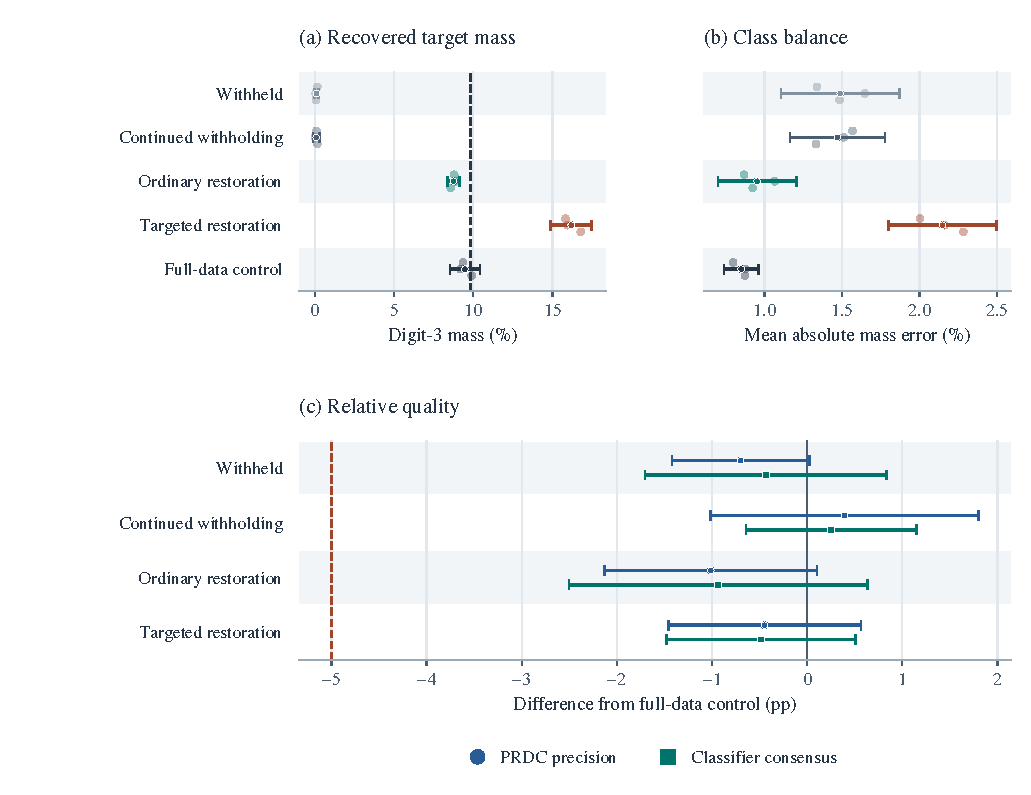
\includegraphics[width=\textwidth]{../figures/mnist_final_primary.pdf}
\caption{Completed original confirmation at DPM++25. All five checkpoint states
and the predeclared quality differences are retained. Small dots show
individual seed outcomes. Intervals are descriptive
95\% Student-$t$ intervals across three independent training seeds; the quality panel's dashed line is the
five-percentage-point noninferiority margin. Ordinary restoration improves
balanced support; targeted restoration overshoots the missing region.}
\label{fig:mnist_primary_supp}
\end{figure*}

\begin{figure*}[t]
\centering
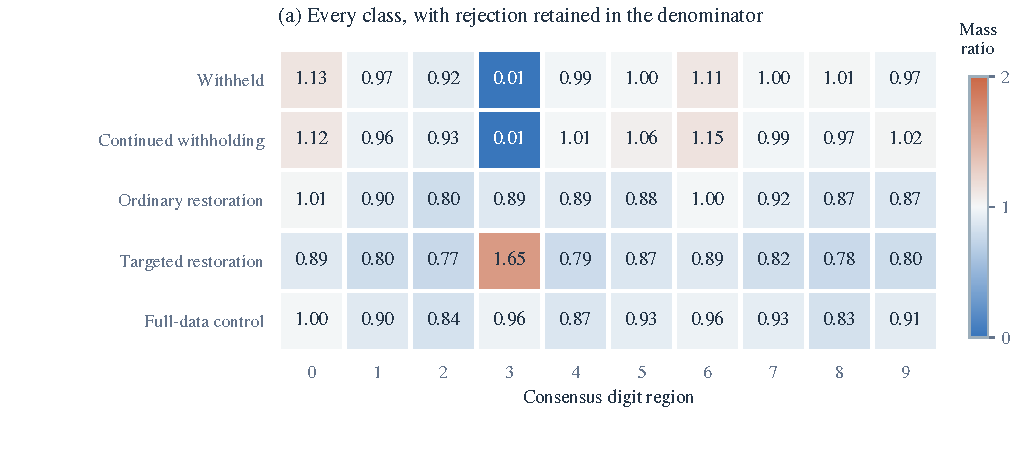
\includegraphics[width=\textwidth]{../figures/mnist_final_class_masses.pdf}
\caption{All ten consensus-region mass ratios relative to real data. This
complete class accounting exposes the targeted intervention's overcorrection.
Rejected samples remain in the denominator; class probabilities are not
renormalized over accepted images.}
\label{fig:mnist_masses_supp}
\end{figure*}

\begin{figure*}[t]
\centering
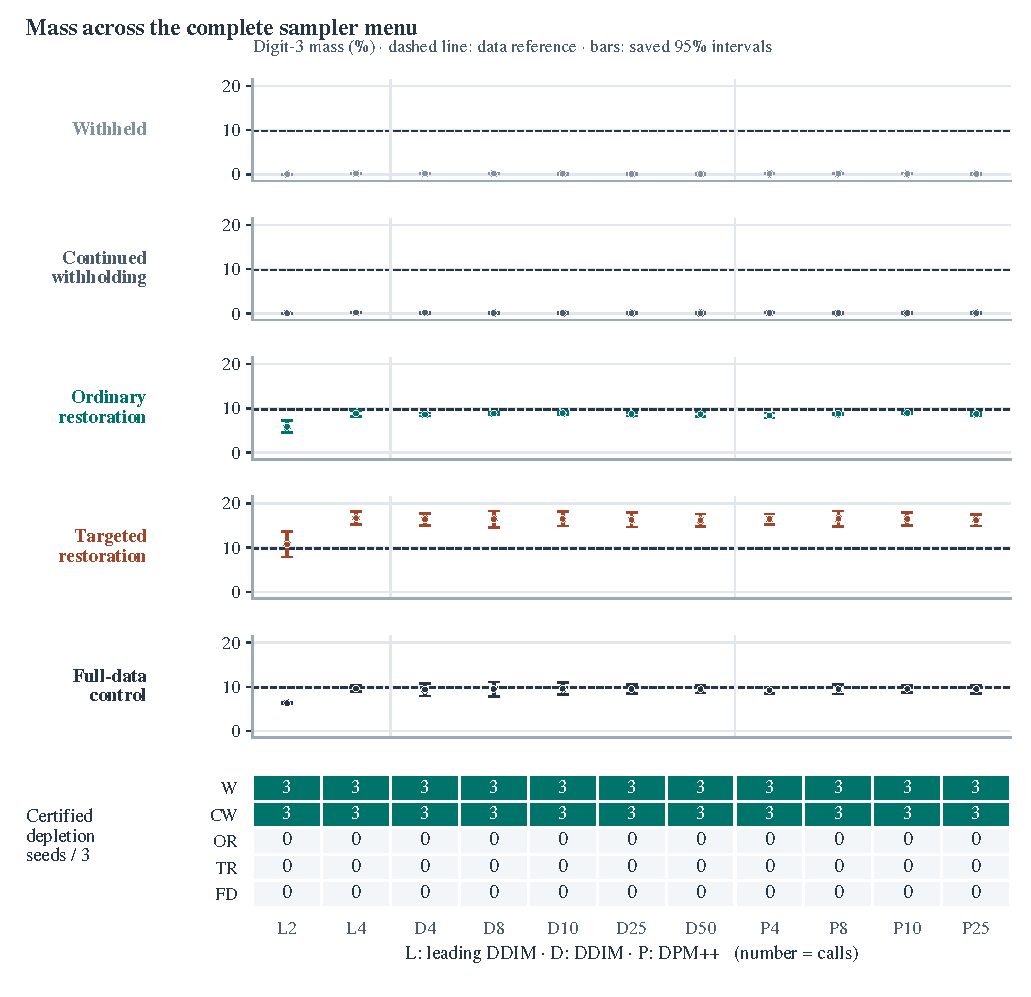
\includegraphics[width=\textwidth]{../figures/mnist_final_solver_persistence.pdf}
\caption{Complete sampler comparison from the original frozen study.
The missing region persists at resolved step budgets under both DDIM and
DPM++, while ordinary data restoration improves its mass. Intervals are
descriptive 95\% Student-$t$ intervals across three training seeds and do not
treat generated panels as independent models.}
\label{fig:mnist_persistence_supp}
\end{figure*}

\begin{figure*}[t]
\centering
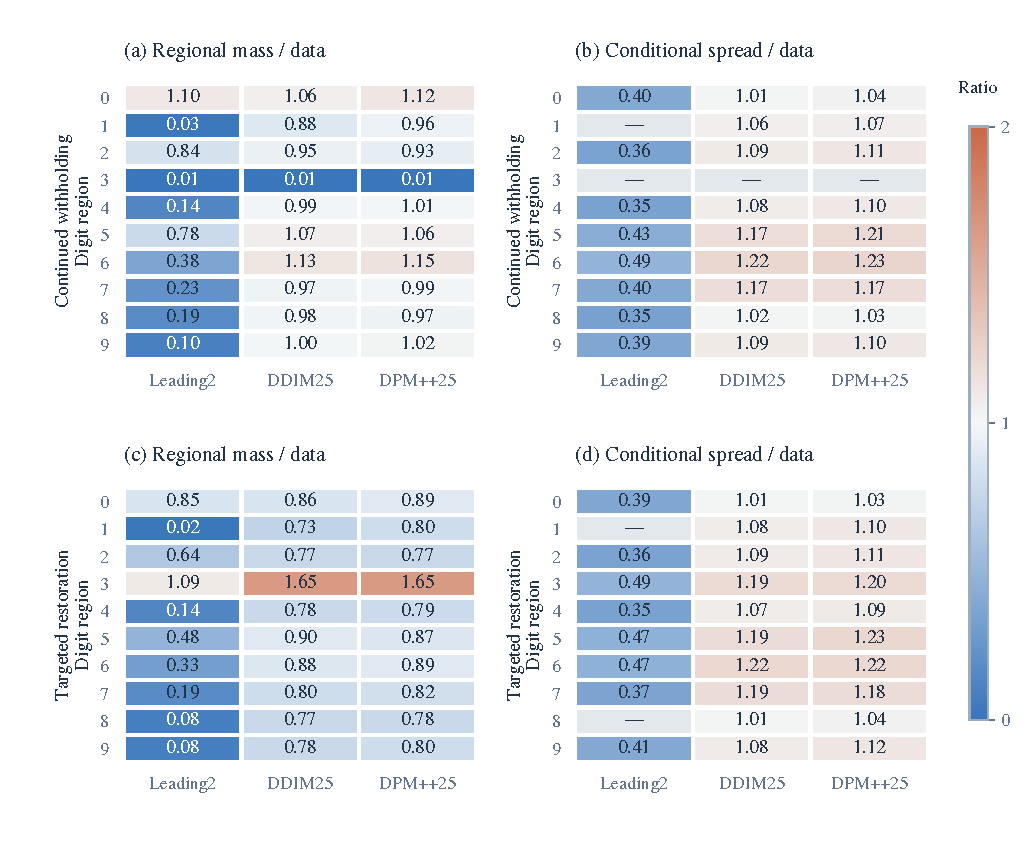
\includegraphics[width=\textwidth]{../figures/mnist_final_mixed_mechanisms.pdf}
\caption{Secondary conditional-spread measurements in independently fitted
PCA32 coordinates and validated semantic cells. Minimum counts and all
ineligible cells are retained. Displayed values are point ratios. Complete interval-based statuses use the
approximate influence-function construction with the declared 1,650-cell
family; they are not exact certificates.}
\label{fig:mnist_mixed_supp}
\end{figure*}

\begin{figure*}[t]
\centering
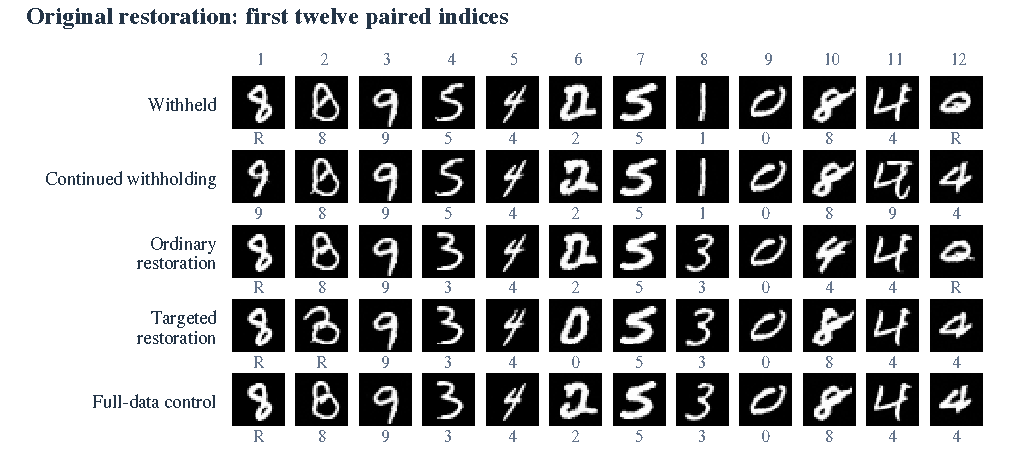
\includegraphics[width=\textwidth]{../figures/mnist_final_qualitative.pdf}
\caption{First twelve noise indices from training seed 10 under DPM++25,
paired across every checkpoint state. No example is ranked or excluded.
Annotations beneath the images show the fixed classifier-consensus digit or rejection; they
allow inspection of the measurement and do not replace visual fidelity.}
\label{fig:mnist_qualitative_supp}
\end{figure*}

\subsection{Signed mass supports an equal-update repair of overcorrection}
\label{sec:mnist_balance_supp}
Ordinary continuation reduces ten-class mass error by 58.7\% and target-digit
absolute error by 89.1\% relative to continued targeting at equal update
budget. This separate follow-up uses a two-sided mass audit to identify
excess probability even when every digit remains represented. Its audit and
matched-update comparison were frozen before follow-up training or generation.
The original restoration results and the 30 crossed-probe routing decisions
(Sec.~\ref{supp:mnist_routing}) remain unchanged. The controlled comparison
tests a repair of measured imbalance without identifying a unique historical cause.

\paragraph{Matched training branches and fresh evaluation.}
Each of the three targeted-restoration checkpoints branches into two further
8,000-update runs. Ordinary continuation draws uniformly from the 60,000
training images. Continued targeted sampling draws from the same images plus
one duplicate of each of the 6,131 digit-3 training images. Both branches
start from identical model, EMA, AdamW, and CUDA random states; the global EMA
counter continues from 33,000 to 41,000 updates. Branch receipts verify these
loaded states. Batch size, learning rate,
optimizer, precision, architecture, and loss are unchanged. No evaluation
occurs during training. The original 33,000-update full-data models are
fixed fidelity controls, not equal-update intervention branches.

All four checkpoint states---targeted parent, ordinary continuation, targeted
continuation, and full-data control---are evaluated under trailing DDIM25,
trailing DDIM50, and second-order DPM++25 for all three training seeds.
Each of these 36 arms receives 16,000 diagnosis samples and 2,000 independent
outcome samples. Noise seeds are paired across arms and are disjoint from
every earlier study. All diagnosis artifacts and their complete decisions
are saved and hashed before outcome generation. Semantic probabilities use
the same frozen classifier-consensus event and all 10,000 real test images;
the denominator includes rejected images. Geometric fidelity retains the
disjoint 3,000/2,000/5,000 real fit/calibration/evaluation split.

\paragraph{Exact two-sided mass bounds.}
For each digit, let $p$ and $q$ be real and generated unconditional consensus
probabilities. We construct Clopper--Pearson intervals $[p_L,p_U]$ and
$[q_L,q_U]$, then report
\begin{equation}
  q-p\in[q_L-p_U,\;q_U-p_L].
\label{eq:supp_mnist_mass_difference}
\end{equation}
The mass error budget is $\alpha_m=0.025$. Half is allocated once across
the ten shared real-reference intervals, and half across all 360 generated
digit--arm intervals. Thus each reference tail has error
$\alpha_m/(4\cdot10)$ and each generated tail
$\alpha_m/(4\cdot360)$. A union bound gives simultaneous coverage at least
$1-\alpha_m$ for the declared differences, conditional on the fixed
semantic regions and trained models. Shared references and paired-noise
dependence across arms do not invalidate this bound.

At the prespecified absolute tolerance $\delta=0.03$, a class is excessive if
the difference interval lies above $\delta$, depleted if it lies below $-\delta$,
equivalent if it lies wholly within $[-\delta,\delta]$, and otherwise inconclusive.
Three percentage points is an explicit MNIST-scale practical resolution,
about 30\% of a nominal balanced class; it is not a universal semantic
threshold. Every class is retained, and the same intervals are evaluated
at $\delta=0.02$ and $0.04$ for sensitivity. Rejection is governed by fidelity,
not treated as a semantic digit.

Synthetic sample planning preceded training. Across 20,000 multinomial
trials per setting, 16,000 generated samples with the fixed-size 10,000-image
reference detect a digit-3 mass of 0.16 as excessive with 99.23\% probability
([99.10,99.35]\% Monte Carlo interval)
and certify all-ten-class equivalence at exactly matching probabilities
with 95.58\% probability ([95.29,95.86]\%). At a digit-3 mass of 0.087,
all-class equivalence power is only 45.12\% ([44.42,45.81]\%); inconclusive
decisions remain expected near the resolution boundary. These planning
calculations concern one sampler, not the three-probe intersection. Its
power also depends on dependence across probes. They are not measured model
performance.

\paragraph{Qualification and persistence.}
The two relative-fidelity events are membership in fixed real-fit
five-neighbor balls and classifier-consensus acceptance. All 27 non-control
arms are paired with the same-seed, same-sampler full-data control. The exact
paired Bernoulli construction in Sec.~\ref{supp:mnist_paired_quality} uses $\alpha_f=0.0125$ across 54 metric
comparisons and a five-percentage-point noninferiority margin. Full-data
self-comparisons are structural zero-difference reference anchors; they do
not establish absolute perceptual fidelity. A checkpoint receives a
persistent-imbalance decision only when at least one same digit is excessive
or depleted under all three resolved samplers and all their fidelity gates
pass. Balanced-at-resolution requires every digit to be equivalent under
all three samplers with the same qualification. All other outcomes are
inconclusive. The calibrated real-support tail is separately reported with
$\alpha_s=0.0125$ across 36 comparisons; it is not silently added as a third
qualification gate. The three exact families sum to 0.05. This simultaneous
statement does not include the approximate training-seed outcome intervals.

\paragraph{Prespecified independent outcomes.}
The two primary comparisons are ordinary minus targeted continuation under
DPM++25 for ten-class mean absolute mass error and digit-3 absolute mass
error. Each receives a 97.5\% paired Student-$t$ interval across the three
training seeds (Bonferroni correction for two comparisons, two degrees of
freedom). These intervals assume approximately normal seed effects and
condition on the common fixed real reference. All other sampler, class,
coverage, precision, support, and variance measurements are reported with
descriptive uncertainty. Four five-percentage-point fidelity constraints
compare ordinary continuation with both continued targeting and the
full-data control for the two declared events; the conjunction passes only
if every paired 95\% interval has lower bound at least $-0.05$.
The 2,000-image outcomes issue no new semantic certificates and do not tune
thresholds, select a sampler, or change diagnosis decisions.

\paragraph{Complete frozen diagnosis.}
The signed audit certifies persistent digit-3 excess in all three targeted
parents and all three continued-targeting checkpoints at $\delta=0.03$.
Digit~3 is equivalent within the same tolerance in all nine ordinary-
continuation probe arms and all nine full-data probe arms. Thus the
specifically identified regional excess is resolved at the declared
resolution, while broader balance remains a separate question.
Every non-control arm passes both relative-fidelity gates (27/27), while
the nine full-data arms retain their explicit anchor status. Ordinary
continuations and full-data controls are all inconclusive for all-ten-class
balance at this resolution; none is labeled data-adequate. At $\delta=0.04$,
ordinary and full-data checkpoints from seeds 10 and 11 receive equivalence
certificates, while both seed-12 checkpoints remain inconclusive. The
seed-10 targeted parent becomes inconclusive for excess at this larger
margin; the other five targeted checkpoints retain persistent excess.
At $\delta=0.02$, the six targeted checkpoints retain excess and the other six
remain inconclusive. Table~\ref{tab:mnist_balance_diagnosis} includes every
checkpoint and sensitivity decision.

The separate support-tail gate passes in 34 of 36 arms. Its two inconclusive
cases are seed-10 targeted-parent DDIM50 and seed-11 full-data DDIM50, with
excess-tail differences 0.03129 [0.01047,0.05085] and
0.03066 [0.00987,0.05020], respectively, against the 0.05 margin.
Neither is a support failure, and neither is silently counted as a pass.
An independent reconstruction of raw semantic counts, paired-fidelity
discordances, support events, and all declared interval/decision formulas
matches the saved diagnosis in all 653 numerical comparisons.

\begin{table*}[t]
\centering\small
\caption{Every signed-mass checkpoint decision. E/D denotes persistent excess/depletion of the listed digit across all three resolved samplers; B denotes all-ten-digit equivalence at the stated resolution; ? denotes inconclusive. Fidelity lists the two-gate conjunction for DDIM25/DDIM50/DPM++25: P (pass), F (fail), I (inconclusive), A (structural reference anchor). Anchors do not certify absolute quality. The primary absolute mass tolerance is $\delta=0.03$; the other columns use the same bounds for prespecified sensitivity analysis.}
\label{tab:mnist_balance_diagnosis}
\begin{tabular}{llcccc}
\toprule
Checkpoint & Seed & Fidelity (25/50/DPM) & $\delta=0.02$ & $\delta=0.03$ & $\delta=0.04$ \\
\midrule
Targeted parent & 10 & P/P/P & E(3) & E(3) & ? \\
Ordinary continuation & 10 & P/P/P & ? & ? & B \\
Targeted continuation & 10 & P/P/P & E(3) & E(3) & E(3) \\
Full-data anchor & 10 & A/A/A & ? & ? & B \\
Targeted parent & 11 & P/P/P & E(3) & E(3) & E(3) \\
Ordinary continuation & 11 & P/P/P & ? & ? & B \\
Targeted continuation & 11 & P/P/P & E(3) & E(3) & E(3) \\
Full-data anchor & 11 & A/A/A & ? & ? & B \\
Targeted parent & 12 & P/P/P & E(3) & E(3) & E(3) \\
Ordinary continuation & 12 & P/P/P & ? & ? & ? \\
Targeted continuation & 12 & P/P/P & E(3) & E(3) & E(3) \\
Full-data anchor & 12 & A/A/A & ? & ? & ? \\
\bottomrule
\end{tabular}
\end{table*}


\paragraph{Independent outcomes and retained tradeoffs.}
Both prespecified primary comparisons favor ordinary continuation.
At DPM++25, ten-class mass error is 0.00900 versus 0.02177 for continued
targeting; the paired difference is $-0.01277$
[$-0.01878,-0.00676$]. Digit-3 absolute error is 0.00747 versus 0.06837,
with difference $-0.06090$ [$-0.11814,-0.00366$]. These are the two
97.5\% adjusted three-seed intervals. The corresponding class-3 masses are
0.09083 and 0.16667 against the real reference's 0.0983. The complete
DDIM25 and DDIM50 comparisons agree in direction: ordinary-minus-targeted
mass-error changes are $-0.01268$ [$-0.01546,-0.00990$] and
$-0.01227$ [$-0.01551,-0.00903$], and class-3 absolute-error changes are
$-0.06173$ [$-0.09812,-0.02534$] and
$-0.06140$ [$-0.09922,-0.02358$]. These secondary intervals are descriptive
95\% intervals, without a simultaneous all-sampler claim.

The four primary fidelity constraints pass. Ordinary-minus-targeted
fixed-neighborhood precision is $+0.00650$ [$-0.00336,0.01636$], while
consensus acceptance changes by $-0.00617$ [$-0.02481,0.01248$].
Against full-data controls, the corresponding changes are $+0.00683$
[$-0.00388,0.01754$] and $+0.00117$ [$-0.03085,0.03318$]. Every lower
bound exceeds $-0.05$. Ordinary continuation has consensus acceptance
0.87383, versus 0.88000 for continued targeting, 0.87267 for full-data
controls, and 0.95460 for real data. The relative-fidelity comparison does
not erase this real/generated difference. Classifier rejection contributes
to the unresolved all-class balance shown in
Fig.~\ref{fig:mnist_balance_allclass}.

Conventional PRDC yields additional, less decisive comparisons. At DPM++25,
ordinary-minus-targeted precision is $-0.00600$ [$-0.02111,0.00911$], and
coverage is $+0.00393$ [$-0.02911,0.03698$]. Thus the mass repair does not
establish broad quality or coverage superiority. PRDC uses the independent
5,000-image real evaluation pool against 2,000 generated outcomes; fixed-
neighborhood precision instead uses 3,000 real-fit anchors. Neither is the
original 165-arm study's five disjoint 1,000-image PRDC panels, so these
absolute values should not be compared across studies without that distinction.
Table~\ref{tab:mnist_balance_all} and the result files retain all 36 arms,
every class, all six checkpoint-pair comparisons under each sampler, and
their three-seed intervals.

\paragraph{Compute and verification.}
The six branches use 48,000 new optimizer updates, or 6.144 million training
batch examples. Three paired workers complete training in approximately
22.4 minutes while sharing an H200; their summed elapsed times are 4,028.7
seconds and are not an exclusive-GPU measurement. Diagnosis generates
576,000 images using 19.2 million denoiser-image calls; independent outcomes
generate 72,000 images using 2.4 million calls. Recorded sampling times are
882.5 and 113.9 seconds, respectively, and CPU diagnosis takes 79.7 seconds.
Per checkpoint, the audit requires 48,000 diagnosis images and 1.6 million
calls across three probes. It is an amortizable checkpoint audit, not a
cheap per-image operation. Generation moves to the second H200 only after
an unrelated old-checkpoint parity check produces exactly identical images,
features, and probabilities on both devices, with all numerical settings
unchanged. Timing is descriptive under concurrent workloads.

The manifest verifies all 72 archives, checkpoint/protocol identities, and
paired seeds. Independent reconstruction matches all 1,661 outcome
comparisons, including PRDC, within $1.78\times10^{-15}$.
Figure~\ref{fig:mnist_balance_grid} retains every state's first twelve
paired outcome seeds.

\begin{table*}[t]
\centering\small\setlength{\tabcolsep}{4pt}
\caption{Complete balance-follow-up outcome comparisons. Mean $\pm$ descriptive 95\% across-training-seed interval half-width ($n=3$); mass metrics use the same 10,000-image semantic reference. Fixed-reference precision uses the original 3,000 real feature anchors. The ordinary and targeted continuation branches each receive 8,000 additional updates from identical targeted parents. Full unrounded endpoints are retained in the result files.}
\label{tab:mnist_balance_all}
\begin{tabular}{llrrrr}
\toprule
Checkpoint & Sampler & Digit-3 mass & Mass MAD $\downarrow$ & Fixed precision $\uparrow$ & Consensus $\uparrow$ \\
\midrule
Targeted parent & DDIM25 & $0.1597\pm0.0268$ & $0.0224\pm0.0064$ & $0.8855\pm0.0120$ & $0.8537\pm0.0186$ \\
Targeted parent & DDIM50 & $0.1592\pm0.0267$ & $0.0216\pm0.0070$ & $0.8845\pm0.0164$ & $0.8618\pm0.0136$ \\
Targeted parent & DPMPP25 & $0.1597\pm0.0225$ & $0.0209\pm0.0044$ & $0.8803\pm0.0134$ & $0.8687\pm0.0029$ \\
Ordinary continuation & DDIM25 & $0.0910\pm0.0087$ & $0.0106\pm0.0048$ & $0.8967\pm0.0133$ & $0.8578\pm0.0318$ \\
Ordinary continuation & DDIM50 & $0.0912\pm0.0148$ & $0.0098\pm0.0046$ & $0.8972\pm0.0107$ & $0.8670\pm0.0305$ \\
Ordinary continuation & DPMPP25 & $0.0908\pm0.0121$ & $0.0090\pm0.0047$ & $0.8965\pm0.0126$ & $0.8738\pm0.0320$ \\
Targeted continuation & DDIM25 & $0.1673\pm0.0284$ & $0.0233\pm0.0054$ & $0.8923\pm0.0047$ & $0.8640\pm0.0281$ \\
Targeted continuation & DDIM50 & $0.1668\pm0.0252$ & $0.0221\pm0.0063$ & $0.8920\pm0.0126$ & $0.8765\pm0.0200$ \\
Targeted continuation & DPMPP25 & $0.1667\pm0.0298$ & $0.0218\pm0.0074$ & $0.8900\pm0.0062$ & $0.8800\pm0.0209$ \\
Full-data control & DDIM25 & $0.0962\pm0.0155$ & $0.0113\pm0.0024$ & $0.8905\pm0.0037$ & $0.8537\pm0.0137$ \\
Full-data control & DDIM50 & $0.0963\pm0.0187$ & $0.0105\pm0.0038$ & $0.8948\pm0.0115$ & $0.8685\pm0.0218$ \\
Full-data control & DPMPP25 & $0.0932\pm0.0127$ & $0.0098\pm0.0034$ & $0.8897\pm0.0117$ & $0.8727\pm0.0093$ \\
\bottomrule
\end{tabular}
\end{table*}


\begin{figure*}[t]
\centering
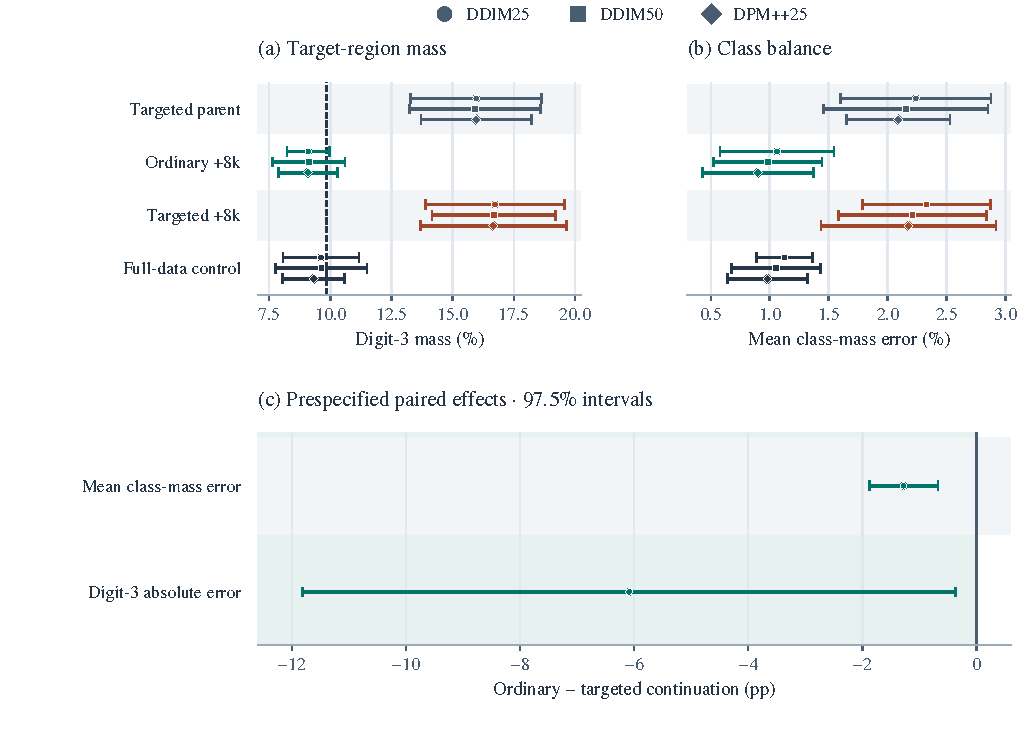
\includegraphics[width=\textwidth]{../figures/mnist_balance.pdf}
\caption{Complete balanced-restoration outcome comparisons.
(a,b) All four checkpoint states and all three resolved samplers, with
descriptive 95\% intervals across three training seeds. The dashed line is
the real digit-3 consensus mass.
(c) Both prespecified DPM++25 differences with 97.5\% paired intervals
(two-comparison adjustment). Intervals condition on the shared fixed real
reference and use the approximate three-seed Student-$t$ model.}
\label{fig:mnist_balance_results}
\end{figure*}

\begin{figure*}[t]
\centering
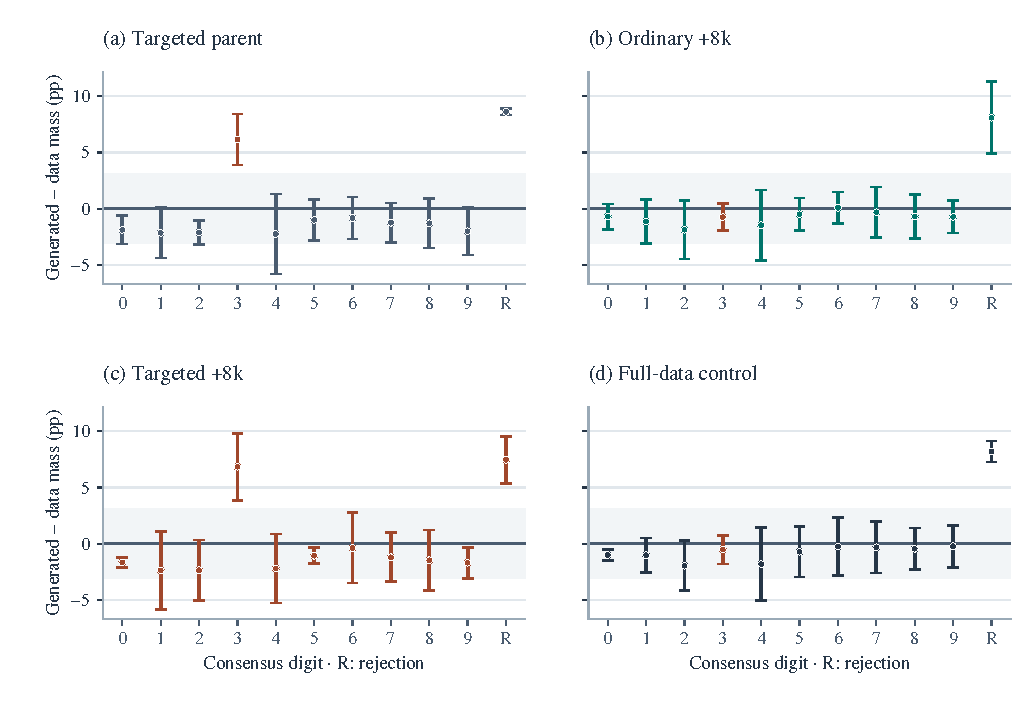
\includegraphics[width=\textwidth]{../figures/mnist_balance_allclass.pdf}
\caption{Every class and the rejection cell at the prespecified DPM++25
sampler. Points are generated-minus-real unconditional masses; intervals
are descriptive 95\% Student-$t$ intervals across three seeds. Digit~3 is
highlighted; the pale band marks the $\pm3$ percentage-point tolerance for
context. These outcome intervals are distinct from the exact diagnosis
bounds. Ordinary continuation resolves the targeted digit's excess while
other regional differences and excess rejection remain visible.}
\label{fig:mnist_balance_allclass}
\end{figure*}

\begin{figure*}[t]
\centering
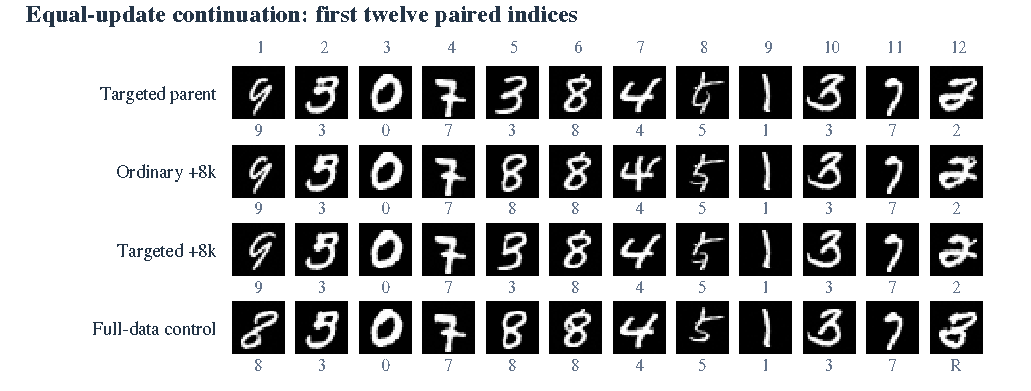
\includegraphics[width=\textwidth]{../figures/mnist_balance_qualitative.pdf}
\caption{Uncurated balanced-restoration outcomes: the first twelve fresh
DPM++25 noise seeds for training seed 10, paired across all four checkpoint
states. The two continuation branches each receive 8,000 updates from the
same targeted parent. The separately trained full-data model is a quality
control. Ambiguous images remain in the grid; none is selected by quality
or classifier label.}
\label{fig:mnist_balance_grid}
\end{figure*}

\begin{figure}[t]
\centering
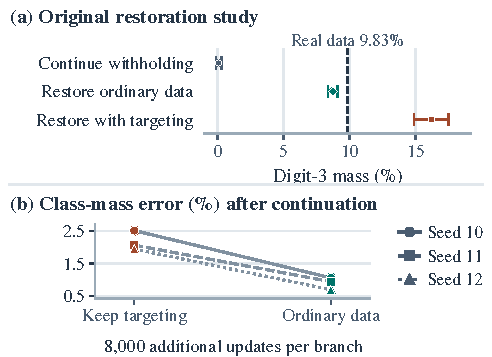
\includegraphics[width=\linewidth]{../figures/mnist_actionable.pdf}
\par\smallskip{\small
\setlength{\tabcolsep}{2.2pt}
\begin{tabular*}{\linewidth}{@{\extracolsep{\fill}}lrrrrr@{}}
\toprule
& \multicolumn{3}{c}{(a) Digit-3 mass (\%)}
& \multicolumn{2}{c@{}}{(b) Class-mass error (\%)} \\
\cmidrule(lr){2-4}\cmidrule(l){5-6}
Seed & Withheld & Ordinary & Targeted & Targeted & Ordinary \\
\midrule
10 & $0.100$ & $8.800$ & $15.820$ & $2.515$ & $1.062$ \\
11 & $0.000$ & $8.860$ & $15.940$ & $2.065$ & $0.946$ \\
12 & $0.160$ & $8.580$ & $16.780$ & $1.950$ & $0.691$ \\
\midrule
Mean & $0.087$ & $8.747$ & $16.180$ & $2.177$ & $0.900$ \\
\bottomrule
\end{tabular*}
}

\caption{Signed measurements support a verified repair of overcorrection.
Both panels use DPM++25. (a) Original ordinary restoration recovers missing
digit-3 mass; targeted restoration overshoots the real-data target (dashed
line). Whiskers show ordinary 95\% Student-$t$ intervals over three training
seeds. (b) A separately frozen follow-up compares equal 8,000-update branches
from each targeted parent. Lines join outcomes from the same seed.
The table gives seed-level values and means.}
\label{fig:mnist_actionable}
\end{figure}

\subsection{Crossed numerical and data probes}
\label{supp:mnist_routing}
The original experiment crosses five checkpoint states with eleven samplers.
We additionally freeze a prospective routing evaluation before generating new
samples. It reuses the three trained seeds and all five states, with leading
DDIM2, trailing DDIM4/25/50, and DPM++25. Each of these 75 arms generates
8,000 diagnosis images and then 2,000 independent outcome images. Every
image uses noise seed $71{,}000{,}000+100{,}000s+i$, with indices 0--7,999
for diagnosis and 8,000--9,999 for outcomes; indices are paired across states
and samplers. All diagnostic routes and policy actions are saved before any
outcome generation begins. No checkpoint is trained further for this study.

\paragraph{Two references and fixed measurements.}
For each short sampler, the same checkpoint's DPM++25 output is its
teacher-relative reference. The data reference uses the final 5,000 real test
images; the first 3,000 fit the geometry and the next 2,000 calibrate its
support threshold. Semantic regions remain the validated classifier-consensus
cells. A fixed real-neighborhood precision event accepts a generated feature
inside the union of real-fit feature balls, each with its fifth-neighbor
radius. This makes each image's precision indicator independent of other
generated images, enabling a paired Bernoulli interval. It differs from
sample-dependent recall and coverage; complete conventional PRDC metrics are
also reported on outcomes.
The fresh outcome PRDC compares 2,000 generated images against all 5,000
reference-evaluation images. This differs from the original study's five
1,000-by-1,000 PRDC panels and its 10,000-image semantic reference. Fresh
semantic masses use only the 5,000 evaluation reference images. Consequently,
absolute nearest-neighbor metrics and finite-reference class masses should
not be compared across the two protocols as if their evaluation sets matched.

\paragraph{Exact paired quality intervals.}\label{supp:mnist_paired_quality}
For each shared-noise pair, let $D=I_{\rm candidate}-I_{\rm reference}$
for consensus acceptance or fixed real-neighborhood precision. Write
$\eta=\Pr(D\ne0)$ and $\pi=\Pr(D=1\mid D\ne0)$. Then the quality
difference is $\Delta=\eta(2\pi-1)$. Clopper--Pearson intervals for
$\eta$ and $\pi$, with tail error $\alpha/(4M)$, give a rectangle;
the minimum and maximum of $\eta(2\pi-1)$ over its four corners bound
$\Delta$. Conditional binomial coverage holds for every random discordance
count, so a union bound proves simultaneous coverage over the declared family.
For zero discordances, the conditional interval is $[0,1]$, giving
$[-\eta^+,\eta^+]$. Both quantities are bounded rather than substituting
a potentially invalid plug-in discordance estimate~\cite{newcombe1998paired};
we do not propose a new paired-proportion estimator.
The same finite-sample calculation is applied to full-data identity controls.
Noninferiority passes only when the lower bound is at least $-0.05$.
Synthetic multinomial simulations and an independent implementation validate
coverage, boundary behavior, and interval arithmetic before learned-model
sampling. At 8,000 pairs, 20,000 synthetic trials with reference acceptance 0.85,
a $-0.01$ difference, and discordance 0.255 give 99.17\% passing probability
(95\% simulation interval 99.03--99.29\%). A $-0.025$ difference gives only
37.91\% power: acceptable differences nearer the margin can remain inconclusive.

\paragraph{Frozen families and route.}
The semantic family contains 1,155 cells: 30 short/data, 30 short/teacher,
and 45 resolved/data comparisons, each with eleven cells and total error
0.025. The paired fidelity family has 150 metric comparisons: the 45 resolved
arms against full-data at the same sampler, plus the 30 short/teacher pairs,
each with two metrics and error 0.0125. Separately, 75 absolute data-support
and 30 paired teacher-support comparisons share error 0.0125. These three
exact families sum to 0.05. Conditional spread uses 300 separately labeled
approximate intervals, one per digit in each short/teacher pair, in unwhitened
PCA32 coordinates. Its paired influence function preserves shared-noise
covariance even when the two samples enter different semantic cells.

A resolved probe is adequate only if both fidelity metrics pass relative to
the corresponding full-data sampler. A data route requires the same digit's
certified depletion under all three resolved probes and adequacy of all three.
A numerical route requires an adequate DPM++25 teacher and short/teacher
regional depletion, conditional contraction, fidelity failure, or support-tail
failure. Both signals produce a combined route; neither yields inconclusive.
Reject-cell depletion does not establish a missing semantic region. Absolute
real-support flags remain visible, including defects shared by the full-data
benchmark; they are not silently promoted to an additional eligibility test.
Because numerical routing can use approximate spread intervals, the entire
routing decision is not an exact 95\% certificate. These are qualified
recommendations for intervention tests, not unique causal identifications.

\paragraph{All policies and independent outcomes.}
For the six original-withheld cases, available data interventions are precisely
the equal-8,000-update continuation branches. A numerical route chooses
continued withholding with DPM++25; a data route chooses ordinary restoration
with the original short sampler; a combined route chooses ordinary restoration
with DPM++25. An inconclusive route uses the continued-withheld short control.
Thus the policy named ``no change'' denotes matched additional training on
withheld data, not the unchanged 25,000-update origin. Comparators are this
control, occupancy-only routing, always numerical, always data, always
combined, targeted restoration at the short sampler, and targeted restoration
with DPM++25. Occupancy-only chooses ordinary restoration whenever any baseline
data-relative digit deficit is certified. All eight policies and all 75 outcome
arms are reported. For every one of the 30 crossed cases we also report the
short-to-DPM++25 outcome change, without inventing a new training transition
from checkpoints that already received restoration.
Numerical repair increases inference cost from 2 or 4 calls to 25; these
comparisons measure the benefit of resolving the sampler, not a free or
matched-budget gain.

Policy intervals average the two short settings within each trained seed,
then use paired Student-$t$ intervals over three seeds. They condition on the
shared real reference and assume approximately normal training-seed effects;
there is no simultaneous superiority claim over policies. The diagnostic
cost is substantial: 600,000 images and 12.72 million denoiser calls across
15 checkpoints, followed by 150,000 independent outcome images. This is a
checkpoint-level audit whose cost can be amortized over deployment, not a
cheap per-prompt diagnostic.
The 8,000 diagnosis samples are per sampler arm: across five samplers this is
40,000 images and 848,000 denoiser-image calls per checkpoint.

\subsection{Crossed-probe outcomes and limits}
All 150 diagnosis/outcome files passed configuration, row-count, pairing,
checkpoint-hash, and sample-checksum validation. The 30 routes were frozen
before any outcome generation. All three resolved probes pass both declared
quality constraints in every checkpoint. The twelve short-sampler cases from
withheld or continued-withheld checkpoints retain the same deficient digit~3
under all three probes and receive the combined route. The eighteen cases from
ordinary restoration, targeted restoration, or full-data training have no
qualified persistent digit depletion and receive the numerical recommendation, which does not certify balanced mass. Training
absence or restoration labels are never inputs to the routing computation.

Occupancy-only routing raises a data flag in nine of the eighteen latter
cases, compared with zero persistent-reference depletion flags. This is a disagreement
in recommendations relative to the known training intervention, not a
classification accuracy or false-positive certificate: targeted restoration,
for example, changes other class probabilities and overrepresents digit~3.
Table~\ref{tab:mnist_all_routes} retains every decision and actual digit counts.
All 30 cases also have exact relative-fidelity evidence for their numerical
signal, although the general rule admits the separately approximate spread
test. No inconclusive outcome occurred in these particular checkpoints;
the implementation and synthetic controls retain that outcome.

The independent short-to-DPM++25 comparison improves class-mass error,
coverage, and consensus acceptance in every one of the eighteen
numerical-only cases. Across ordinary-restored, targeted, and full-data
checkpoints, mean mass-error changes are respectively $-0.05022$, $-0.03783$,
and $-0.05097$ from leading DDIM2, and $-0.01781$, $-0.01772$, and $-0.01804$
from trailing DDIM4. Precision has a meaningful tradeoff: fixed-neighborhood
membership improves from the two-call sampler but decreases from trailing
DDIM4 by 0.01133, 0.02150, and 0.01950, respectively. All 75 arms and all
30 paired changes, including their three-seed intervals, remain in the result
files. These observed numerical improvements use existing checkpoints. They do not
establish that all eighteen checkpoints need no data intervention: the six
targeted-checkpoint cases retain excess digit-3 mass, which the depletion-only
rule does not test. Of the nine nonpersistent occupancy flags, three come
from leading-DDIM2 targeted cases with this distinct imbalance. We therefore
do not count nine correct avoided training interventions or claim measured
counterfactual training savings.

For the six original-withheld origins, the audit chooses ordinary restoration
plus DPM++25 and therefore equals always-combined exactly. Its digit-3 mass is
$0.08567\pm0.01120$, versus $0.00067\pm0.00072$ for numerical repair alone.
Mass error is $0.01162\pm0.00117$, versus $0.04563\pm0.00191$ for data-only
repair and $0.01493\pm0.00379$ for numerical-only repair. Audit-minus-numerical
mass error is $-0.00331$ [$-0.00683,0.00020$], so superiority on this endpoint
is unresolved. Audit-minus-data-only error is $-0.03402$
[$-0.03555,-0.03248$]. Targeted restoration plus DPM++25 again overshoots,
with digit-3 mass 0.1650 and error 0.02348. All eight policies are retained in
Table~\ref{tab:mnist_routing_policies}; these are descriptive paired
three-training-seed comparisons, not a simultaneous best-policy claim.

Sampling takes 924.8 seconds for diagnosis and 221.1 seconds for outcomes;
CPU routing and outcome measurement take approximately 86 and 188 seconds.
No additional training is performed. Figure~\ref{fig:mnist_routing_grid_supp}
retains the first twelve fresh outcome noise indices from seed 10 for every
listed arm, including classifier rejections.

\begin{table*}[t]
\centering\small
\setlength{\tabcolsep}{4pt}
\caption{Fresh routing outcomes. All policies were frozen on independent diagnosis seeds. Mean $\pm$95\% Student-$t$ interval over three trained seeds, averaging the two short settings within each seed. Precision uses the fixed real-neighborhood event. Continued withholding is the matched 8,000-update control. These complete secondary comparisons do not assert simultaneous policy superiority.}
\label{tab:mnist_routing_policies}
\begin{tabular}{lrrrrr}
\toprule
Policy & Digit-3 mass & Mass error $\downarrow$ & Precision $\uparrow$ & Consensus $\uparrow$ & Calls \\
\midrule
Audit & $0.086\pm0.011$ & $0.012\pm0.001$ & $0.894\pm0.009$ & $0.865\pm0.025$ & $25.0$ \\
Occupancy only & $0.076\pm0.013$ & $0.046\pm0.002$ & $0.868\pm0.007$ & $0.517\pm0.019$ & $3.0$ \\
Numerical & $0.001\pm0.001$ & $0.015\pm0.004$ & $0.905\pm0.020$ & $0.875\pm0.010$ & $25.0$ \\
Restore data & $0.076\pm0.013$ & $0.046\pm0.002$ & $0.868\pm0.007$ & $0.517\pm0.019$ & $3.0$ \\
Restore + numerical & $0.086\pm0.011$ & $0.012\pm0.001$ & $0.894\pm0.009$ & $0.865\pm0.025$ & $25.0$ \\
Targeted & $0.137\pm0.017$ & $0.051\pm0.001$ & $0.871\pm0.013$ & $0.534\pm0.023$ & $3.0$ \\
Targeted + numerical & $0.165\pm0.015$ & $0.023\pm0.002$ & $0.888\pm0.013$ & $0.867\pm0.016$ & $25.0$ \\
Continue withheld & $0.001\pm0.001$ & $0.045\pm0.001$ & $0.875\pm0.007$ & $0.527\pm0.008$ & $3.0$ \\
\bottomrule
\end{tabular}
\end{table*}

\begin{table*}[t]\centering\small
\setlength{\tabcolsep}{4pt}
\caption{All 30 fresh depletion-only routing cases. The occupancy flag uses short-sampler data-relative digit depletion; persistence requires the same digit under all three quality-qualified resolved probes. Digit-3 counts are paired short/DPM++25 counts, out of8,000 for diagnosis and2,000 for independent outcomes. N denotes a numerical recommendation and D a data recommendation; N does not certify balanced data-relative mass. Training-state names are reporting labels, not inputs to the rule.}
\label{tab:mnist_all_routes}
\begin{tabular}{llrrrrrrr}\toprule
State & Seed & Calls & Occupancy flag & Persistent flag & Route & Diagnosis 3 & Outcome 3 & $\Delta$ mass error \\\midrule
Withheld & 10 & 2 & 1 & 1 & N+D & 6/8 & 0/3 & -0.0460 \\
Withheld & 10 & 4 & 1 & 1 & N+D & 16/8 & 2/3 & -0.0133 \\
Continue & 10 & 2 & 1 & 1 & N+D & 6/6 & 1/1 & -0.0475 \\
Continue & 10 & 4 & 1 & 1 & N+D & 8/6 & 3/1 & -0.0155 \\
Restore & 10 & 2 & 1 & 0 & N & 509/710 & 140/172 & -0.0483 \\
Restore & 10 & 4 & 0 & 0 & N & 700/710 & 176/172 & -0.0183 \\
Targeted & 10 & 2 & 1 & 0 & N & 902/1312 & 243/344 & -0.0375 \\
Targeted & 10 & 4 & 0 & 0 & N & 1299/1312 & 337/344 & -0.0173 \\
Full & 10 & 2 & 1 & 0 & N & 524/746 & 146/170 & -0.0483 \\
Full & 10 & 4 & 0 & 0 & N & 727/746 & 191/170 & -0.0171 \\
Withheld & 11 & 2 & 1 & 1 & N+D & 9/8 & 2/3 & -0.0463 \\
Withheld & 11 & 4 & 1 & 1 & N+D & 23/8 & 3/3 & -0.0166 \\
Continue & 11 & 2 & 1 & 1 & N+D & 2/11 & 2/2 & -0.0448 \\
Continue & 11 & 4 & 1 & 1 & N+D & 19/11 & 5/2 & -0.0148 \\
Restore & 11 & 2 & 1 & 0 & N & 468/684 & 121/180 & -0.0514 \\
Restore & 11 & 4 & 0 & 0 & N & 682/684 & 194/180 & -0.0170 \\
Targeted & 11 & 2 & 1 & 0 & N & 809/1278 & 199/325 & -0.0378 \\
Targeted & 11 & 4 & 0 & 0 & N & 1312/1278 & 337/325 & -0.0175 \\
Full & 11 & 2 & 1 & 0 & N & 531/768 & 146/192 & -0.0527 \\
Full & 11 & 4 & 0 & 0 & N & 735/768 & 191/192 & -0.0191 \\
Withheld & 12 & 2 & 1 & 1 & N+D & 10/6 & 4/3 & -0.0481 \\
Withheld & 12 & 4 & 1 & 1 & N+D & 13/6 & 3/3 & -0.0144 \\
Continue & 12 & 2 & 1 & 1 & N+D & 8/9 & 1/1 & -0.0469 \\
Continue & 12 & 4 & 1 & 1 & N+D & 12/9 & 4/1 & -0.0134 \\
Restore & 12 & 2 & 1 & 0 & N & 541/702 & 115/162 & -0.0510 \\
Restore & 12 & 4 & 0 & 0 & N & 743/702 & 163/162 & -0.0180 \\
Targeted & 12 & 2 & 1 & 0 & N & 993/1358 & 211/321 & -0.0381 \\
Targeted & 12 & 4 & 0 & 0 & N & 1422/1358 & 321/321 & -0.0183 \\
Full & 12 & 2 & 1 & 0 & N & 543/784 & 113/192 & -0.0519 \\
Full & 12 & 4 & 0 & 0 & N & 834/784 & 187/192 & -0.0179 \\
\bottomrule\end{tabular}\end{table*}


\begin{figure*}[t]
\centering
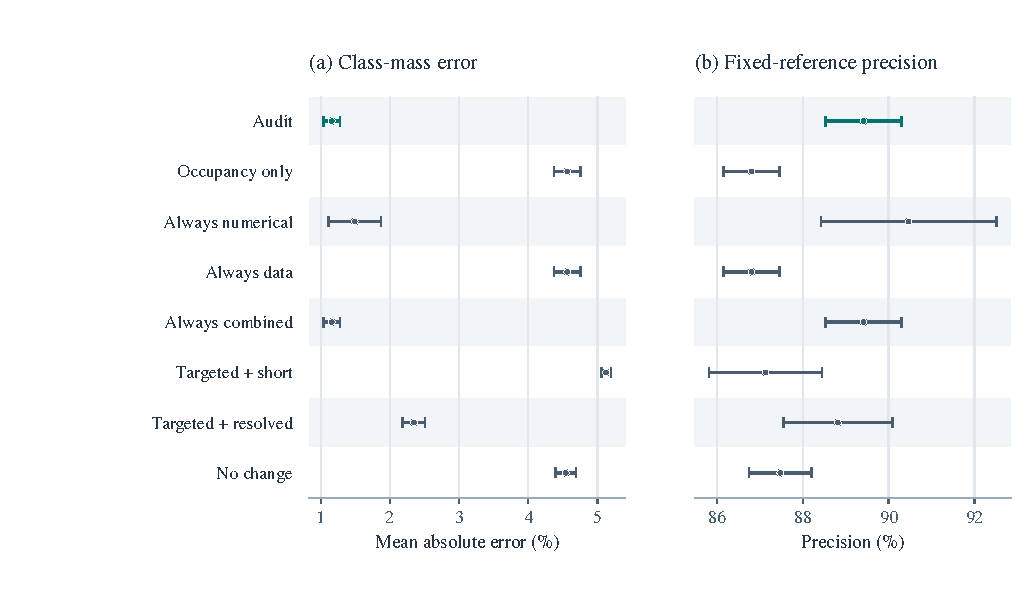
\includegraphics[width=\textwidth]{../figures/mnist_routing.pdf}
\caption{Complete independent outcomes of the depletion-only routing
study: all eight policies for six original-withheld origins. Both short settings
are averaged within each training seed; intervals are descriptive 95\%
Student-$t$ intervals over three seeds. (a) Mean absolute class-mass error.
(b) Membership in fixed real-fit five-neighbor balls. Numerical repair uses
25 calls versus the original 2/4; audit and always-combined coincide.
All 30 frozen recommendations remain in Table~\ref{tab:mnist_all_routes}.
A numerical recommendation does not certify balanced mass.}
\label{fig:mnist_routing}
\end{figure*}

\begin{figure*}[t]
\centering
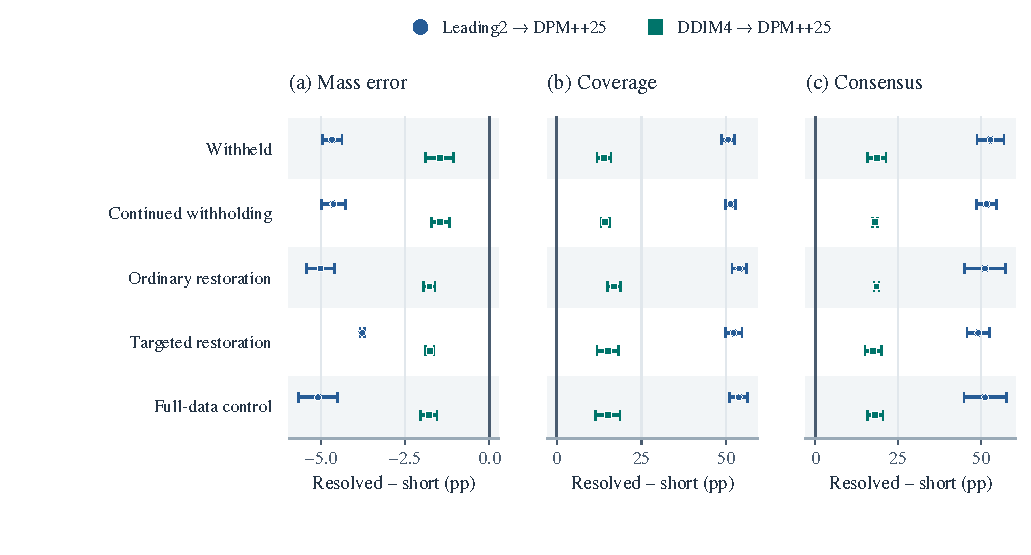
\includegraphics[width=\textwidth]{../figures/mnist_routing_numerical.pdf}
\caption{Every checkpoint state's independent short-to-resolved comparison.
All changes use the same checkpoint and paired fresh noise; intervals are
approximate 95\% paired Student-$t$ intervals across three trained seeds.
Numerical improvement cannot recover the withheld digit's data-relative mass;
restoration is needed for that deficit. Complete precision and support
outcomes accompany these plots in the saved result tables.}
\label{fig:mnist_routing_numerical_supp}
\end{figure*}

\begin{figure*}[t]
\centering
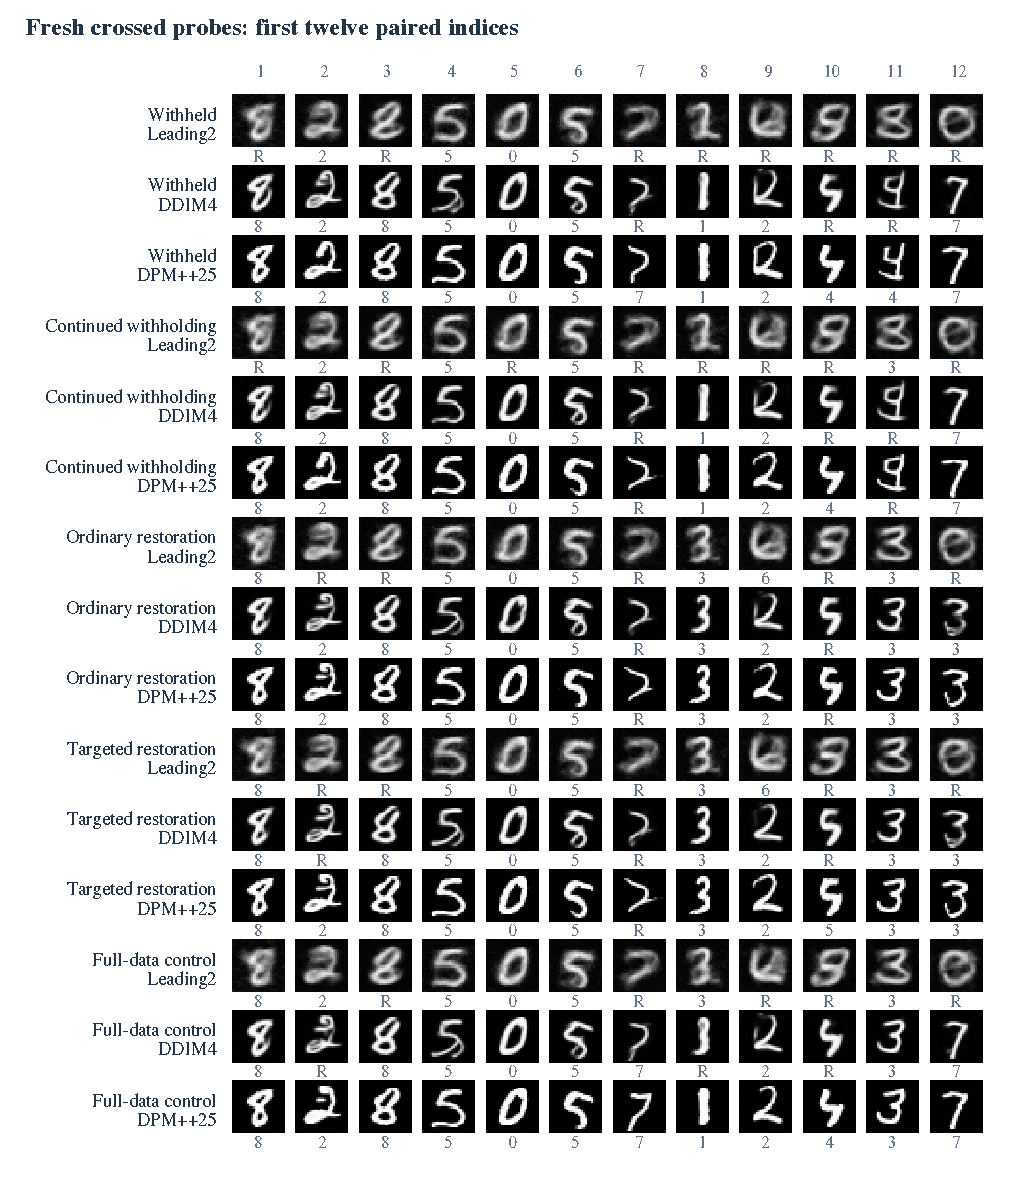
\includegraphics[width=\textwidth]{../figures/mnist_routing_qualitative.pdf}
\caption{Uncurated fresh outcomes: first twelve noise indices of training
seed 10, paired across all five checkpoint states and the two short samplers
plus DPM++25. Labels beneath the images are fixed classifier-consensus assignments or rejection.
Numerical resolution sharpens samples and increases acceptance; restored
data changes which semantic outcomes the checkpoint produces. Imperfect
digits and classifier disagreements remain visible.}
\label{fig:mnist_routing_grid_supp}
\end{figure*}
